\chapter{Predchádzajúce riešenia}\label{chap:previous_solutions}

V nasledujúcej kapitole opíšeme existujúce riešenia, zameriame sa na ich výhody a prípadné nevýhody.

\section{SVGEdit}

SVGEdit je jediné oficiálne rozšírenie MediaWiki existujúce v dobe písania tejto diplomovej práce. Aktuálne ja v stave experimental, čo naznačuje, že nie všetka funkcionalita bude bezproblémová. Poskytuje možnosti vytvárania a editovania súborov vektorovej grafiky vo formáte svg. Využíva open source SVG-edit widget, ktorý poskytuje štandardnú funkcionalitu vektorového editora, s relatívne vysokou kvalitou spracovania. 

Nevýhodou tohoto riešenia je, že samotný editor je vložený formou iframe widgetu zo stránok vývojárov tohoto widgetu. To spôsobuje nemožnosť upraviť vzhľad alebo funkcionalitu editora. Prepojenie s MediaWiki systémom je zabezpečené pomocou asynchrónnych ajax volaní. Editor taktiež nepodporuje kolaboratívnu úpravu jedného súboru viacerými používateľmi. Ďalšou nevýhodou je jeho zložité ovládanie nehodiace sa pre cieľovú skupinu finálnej aplikácie, ktorou sú študenti základných a stredných škôl.

\begin{figure}[h]
	\centerline{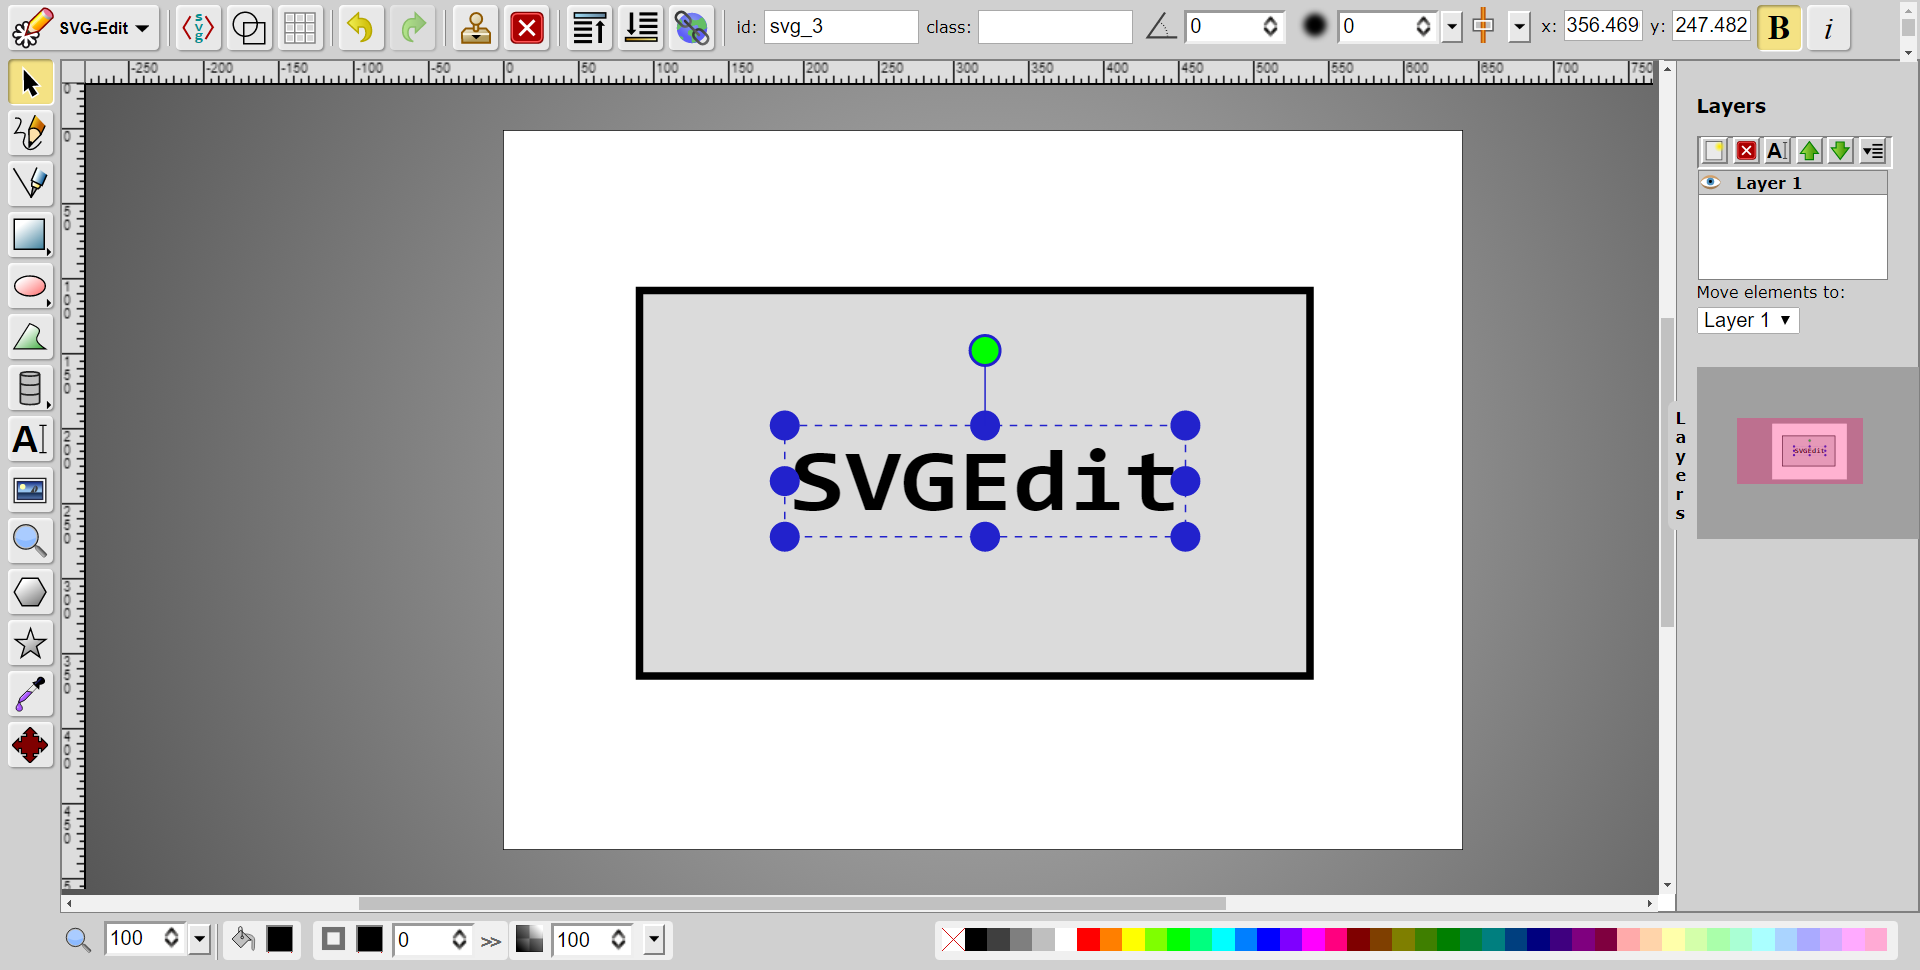
\includegraphics[width=0.8\textwidth]{images/svg-edit}}
	\caption[Editor SVG-edit]{Prostredie editora SVG-edit}
	\label{obr:SVGedit}
\end{figure}
\FloatBarrier


\section{Figma}

Figma je profesionálny grafický editor s možnosťou kolaboratívnej práce viacerých používateľov. Je určený predovšetkým pre ľudí zaoberajúcich sa grafickým návrhom mobilných, webových alebo desktopových aplikácií. Jeho hlavnou výhodou je intuitívne ovládanie, real-time komunikácia medzi spolupracujúcimi používateľmi a bohatá funkcionalita. 

Keďže sa však jedná o samostatnú webovú aplikáciu, nie je možné ju implementovať do MediaWiki systému.

\begin{figure}[h]
	\centerline{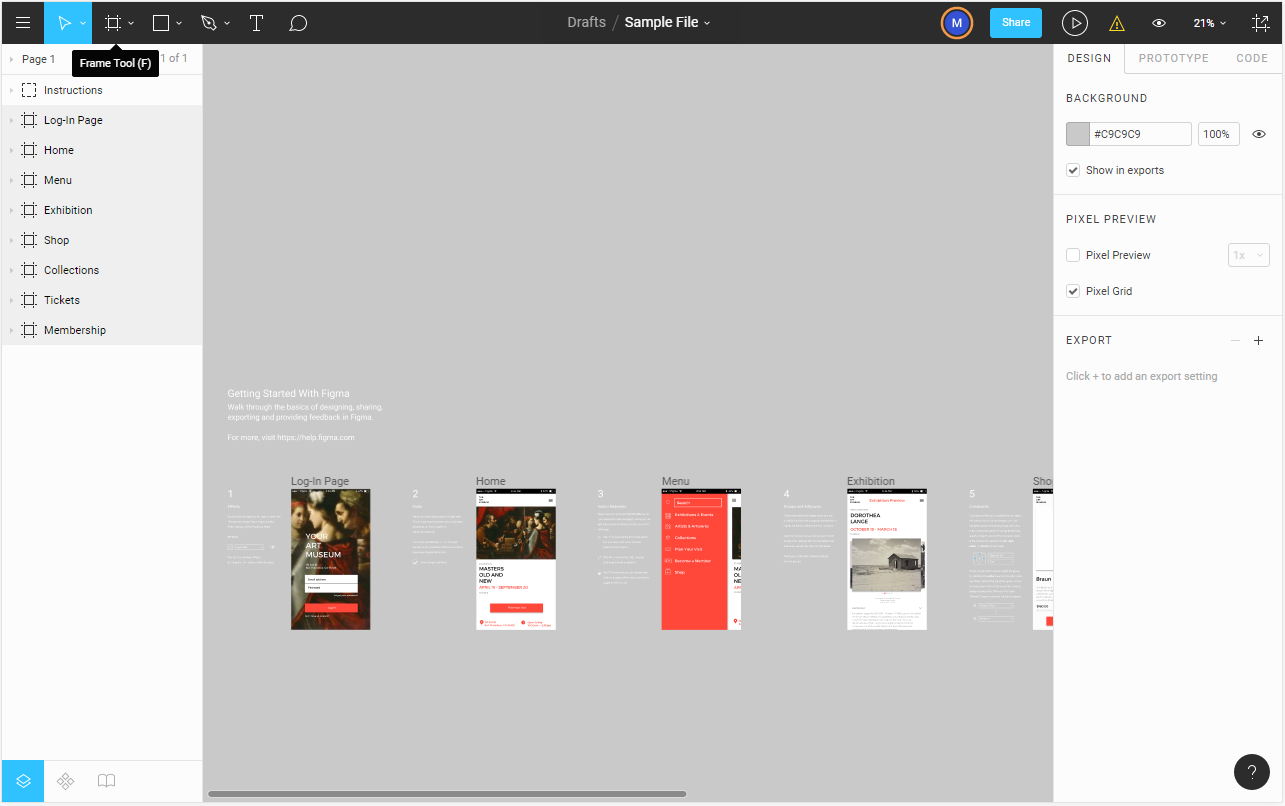
\includegraphics[width=0.8\textwidth]{images/figma}}
	\caption[Editor Figma]{Prostredie kolaboratívneho editora Figma}
	\label{obr:Figma}
\end{figure}
\FloatBarrier

\section{Draw.IO}
\textit{Draw.IO} je online webová aplikácia slúžiaca na kolaboratívnu tvorbu vektorovej grafiky. Využitie tejto aplikácie je možné nájsť najmä pri tvorbe:
\begin{itemize}
	\item \textit{Diagramov} na lepšie pochopenie funkčnosti aplikácie, postupov vývoja alebo dátového modelu. Podporuje tvorbu \textit{UML}, \textit{BPMN}, \textit{stromových}, \textit{sieťových}, \textit{sekvenčných}, \textit{elektrotechnických} a množstva ďalších diagramov.
	\item \textit{Obrysových (wireframe) modelov} na plánovanie rozloženia elementov pri návrhu mobilných, počítačových alebo webových aplikácií.
	\item \textit{Vývojových (mockup) modelov} na rýchle prototypovanie vzhľadu aplikácie.
	\item \textit{Grafov} - Ganttov graf používaný pri plánovaní projektov, zobrazujúci časovú závislosť jednotlivých podúloh.
	\item \textit{Architektonických plánov} podlaží budov.
	\item \textit{Infografiky} na lepšiu zapamätateľnosť informácií.
\end{itemize}
Umožňuje bezplatné prepojenie s viacerými cloudovými riešeniami ako Google Drive, OneDrive alebo možnosť integrovať do vývojových kolaboratívnych softvérov Confluence a Jira. Aplikáciu je možné používať aj pomocou desktopových aplikácií na všetkých bežných operačných systémoch (Windows, macOS, Linux, Chrome OS). 
Ďalšími výhodami sú jednoduché a intuitívne ovládanie, dobrá skálovateľnosť pre projekty s veľkým množstvom elementov, možnosť bezplatného používania a  voľná prístupnosť zdrojových súborov aplikácie pre vývojárov.

Nevýhodou je že aplikáciu nieje možné prepojiť so systémom MediaWiki a nepodporuje voľné kreslenie objektov. Tie môžu byť importované formou obrázka.

\begin{figure}[h]
	\centerline{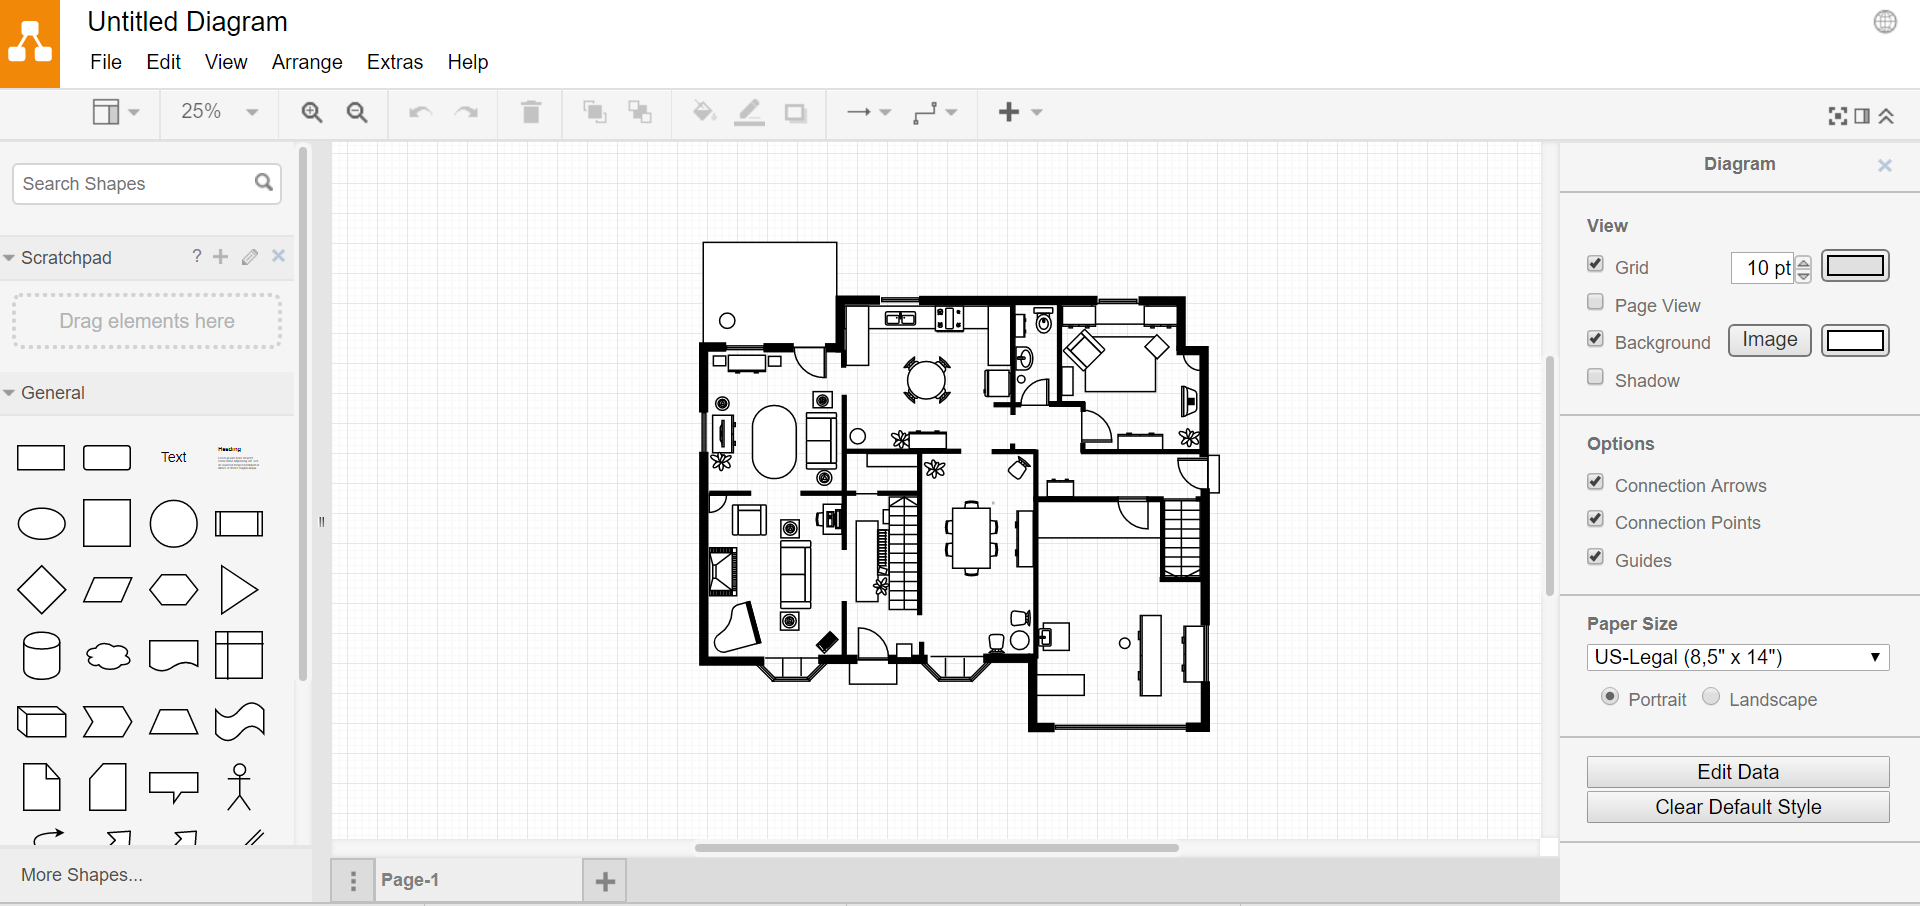
\includegraphics[width=0.8\textwidth]{images/drawio}}
	\caption[Editor Draw.IO]{Prostredie kolaboratívneho editora Draw.IO}
	\label{obr:DrawIO}
\end{figure}
\FloatBarrier